\chapter{Introduction}
A big field in astronomy and particle physics ever since Victor Hess discovered
the extraterrestrial origin of the atmospheric ionization
is astroparticle physics. Despite falling out of favor for a few years
when terrestrial particle accelerators reached ever higher energies,
the field is very famous today. One of the reasons is that
even the biggest accelerators, like the LHC at CERN, got to a point where
increasing collision energies gets ever more difficult.

Despite recent achievements and much research going on
in the field of astroparticle physics
there are still many questions left.
Some of the prominent ones are:
(VLT FÜR DIE ARBEIT RELEVANTERE FRAGEN WÄHLEN? nimm die aus funcray!)
\begin{itemize}
    \item{How does general relativity work with quantum gravity and 
	what happens at the singularities?}
    \item{Which particles form the dark matter?}
    \item{Why is the universe expanding and what is dark energy?}
    \item{How do cosmic rays get accelerated to the highest energies?}
    \item{Are neutrinos majorana particles?}
\end{itemize}

Nowadays there exists a wide range of experiments trying to
solve these questions. They focus on different particles and detection
mechanisms to detect
extraterrestrial particle sources, which is why
the term multi messenger astronomy is widely used.

Besides an overview of the most important findings in the history
of astroparticle physics, we will have a look at the 
most influencal IACT experiments.

\section{The origins of astroparticle physics}
1785 Charles-Augustin de Coulomb first described the electrostatic forces 
and found out that the electric charge on an electroscope can
reduce over time although no contact has been made \cite{coulomb1785premier}.
(Quelle finden und lesen)

Much later, in 1879, William Crookes noted that the speed of the discharge
depended on the pressure of the surrounding air 
\cite{doi:10.1098/rstl.1879.0076}.
This lead to the insight that the air must be ionized, but an 
explanation was not yet available.

A step towards the solution of this mistery was the discovery 
of radioactivity by Henri Becquerel in 1896 
\cite{becquerel1896emission} (finden und lesen)
and the following studies of Marie and Pierre Curie, 
that awarded all three of them the nobel prize \cite{nobel_curie}

With experimental improvements, quantitative measurements
of the spontaneous discharge became possible.
One of multiple contemporaneous experiments was 
led by Charles Thomson Rees Wilson, who also 
acknowledged Geitel and Matteuci to have found the same 
results independently
\cite{doi:10.1098/rspl.1901.0032}.

For this the electroscope was insulated into a closed vessel.
With these measurements it became evident that the source 
of the ionised particles was indeed outside of the vessel.
The obvious explanation seemed to be that the surrounding material 
emitted radioactivity.
Although Wilson proposed a penetrating extraterrestrial radiation, 
he could not support his theory with experimental results, 
so the idea was dropped \cite{bookap}.

By 1909 it was found, that the mysterious radiation was also 
penetrating metal, which only left $\gamma$-radiation as 
possible source. Besides radioactivity in the earth crust or atmosphere,
another possible source was assumed to be the sun \cite{bookap}.

To test these hypotheses, the following years included many experiments 
above or under sea level to measure if the radiation strength changes.

In 1909 Theodor Wulff measured the radiation on top of the 
eiffel tower in paris
\cite{wulf1909atmosphare}. (finden und lesen!)
Assuming that most radiation came from the 
earth crust, the decrease was less than expected.

Balloon flights of Albert Gockel in 1909 
\cite{gockel1909atmosphare} (finden und lesen ggf englische version?)
and underwater experiments of Domenico Pacini in 1910 
\cite{2011arXiv1101.3015P}
lead to the conclusion that most of the radiation must indeed be
of extraterrestrial origin, which was not widely accepted 
in the community though \cite{bookap}.

Evidence came with the extended ballon flights of Victor Hess
\cite{Hess:1912srp}:
Not only was the intensity decrease with higher altitude not 
matching the expectations, but at a certain point at around 
\SI{2000}{\meter} the intensity 
was actually increasing again.
As this was also the case in night flights, the sun
was excluded as possible source.
A few years later, in 1929, Werner Kolhörster and 
Walther Bothe confirmed these experimental results \cite{bothe1929wesen}.

The radiation was referenced as "Höhenstrahlung" 
(see e.g. \cite{myssowsky1926versuche}) 
and "cosmic rays" (see e.g. \cite{millikan1928origin}) with 
the english term cosmic rays eventually winning out.


Since the experiments of Jacob Clay in 1927 
\cite{clay1927penetrating}
it was clear that the main proportion of 
this radiation must carry an electric charge.

With experiments resolving around the influence of the earth magnetic 
field by 
Bruno Rossi \cite{Rossi1933},
Thomas H. Johnson \cite{PhysRev.43.834},
Luis Alvarez and Arthur H. Compton \cite{PhysRev.43.835}
in 1933,
a positive charge was conducted.

The remaining puzzles towards gamma astronomy were 
solved with the discovery of antimatter in a cloud chamber
by Carl D. Anderson in 1933
\cite{PhysRev.43.491}
and the discovery of air showers by detecting coincident 
events in separated geiger-müller tubes by 
Bruno Rossi in 1934
\cite{PhysRev.45.212}
and their later description by
the team around Pierre Auger 
\cite{RevModPhys.11.288}.

In the following years multiple particles with direct use in the 
astrophysics have been found:
The pions \cite{LATTES1947}, the muons \cite{PhysRev.52.1003}
and the neutrinos \cite{Cowan103}.

The so far last discovery on this journey
was the recent measurement of the first gravitational 
waves \cite{PhysRevLett.118.221101}.

\section{Multimessenger astronomy}

Nowadays we observe extraterrestrial processes on four channels: 
\begin{enumerate}
	\item Electromagnetic radiation
	\item (Charged) cosmic rays
	\item $\nu$-radiation
	\item Gravitational waves
\end{enumerate}

All of these have vastly different properties and require different experiments.
A common thing is to observe the same sources 
on different channels to learn more about the processes that happen at 
these far distant sources. This is what is often times 
referred to as multi messenger astronomy (cite some mma paper, eg magic looking at an icecube alert).

Before we focus on the special field of IACTs, we will have
a brief look at the different messenger particles.

\begin{figure}
	\centering
	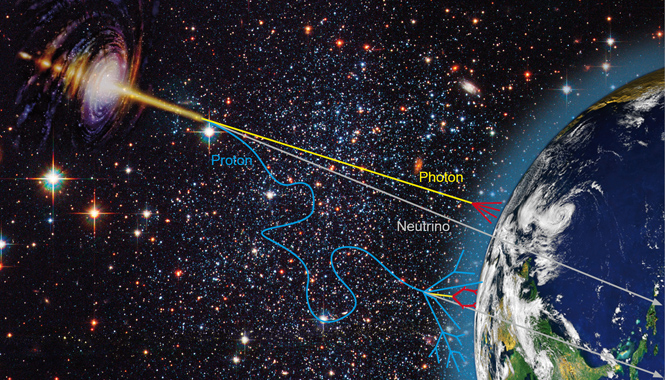
\includegraphics[width=.8\textwidth]{images/astro-web-titel.jpg}
	\label{fig:multi_messenger}
	\caption{Visualisation of the behaviours of different astronomy messengers.
		Photons and neutrinos 
		travel the universe without deflection.
		Charged cosmic rays get deflected by interstellar
		magnetic fields and thus do not allow for a assignment to a cosmological source.
		Neutrinos interact way less than photons both in the universe and in the detector 
		which requires the detectors to be of huge areas and leads to a high 
		proportion passing through earth
		\cite{desy_mm_astro}.
		This illustration lacks gravitational waves 
		as these have only recently been measured and play no relevant role 
		for Imaging Air Cherenkov Telescopes (IACTs).
	}
\end{figure}


\subsection{Charged cosmic rays}
The term charged cosmic rays summates all types of charged particles from
extra terrestrial sources with the main proportion being protons
\cite{Dembinski:2017zsh}.


\begin{figure}
	\centering
	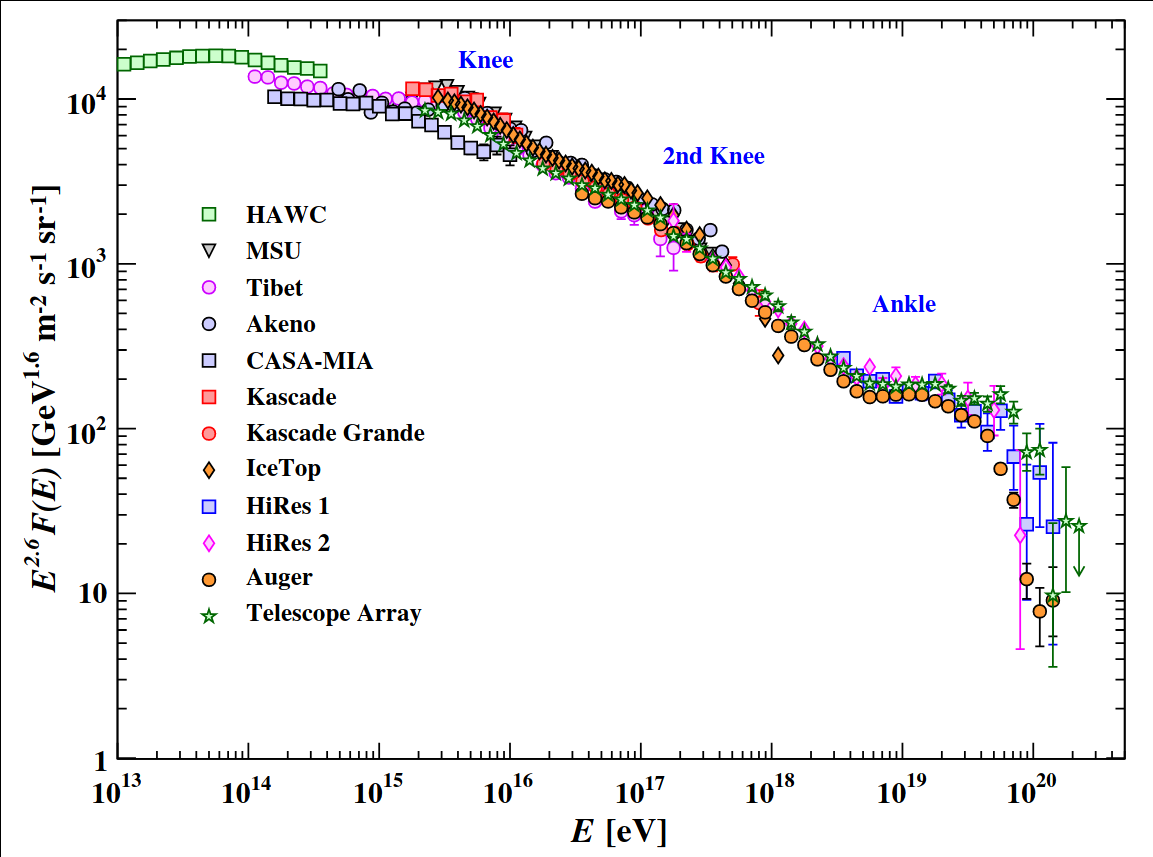
\includegraphics[width=.8\textwidth]{images/cr_spectrum.png}
	\caption{Combined plot of the cosmic ray spectrum,
		measured by different air shower experiments \cite{pdg19}. 
		(original sources? stehen im pdg)
	}
	\label{fig:cr_spectrum}
\end{figure}

Figure \ref{fig:cr_spectrum} shows the flux of charged cosmic rays over 
many orders of magnitude in energy which mainly follows 
a power law $E^{-\gamma}$ with $\gamma$ somewhere between 
2.7 and 3.3. Deviations from this crude approximation are 
usually referred to as the first and second knee and the ankle 
at $\num{5e15}, \num{2e17}$ and $\SI{5e18}{\electronvolt}$ respectively.
At the very highest energies, the flux seems to rapidly decrease,
which may point towards a maximum energy
that cosmological sources can produce or towards destructive interaction with 
the cosmic microwave background \cite{bookap}.

The current model assumes the high energy cosmic rays to be produced 
mainly in supernova remnants (SNRs) through the expanding shock waves.

An important description of the acceleration process has been
worked out by Enrico Fermi in 1949 \cite{PhysRev.75.1169}.
The main assumption is that the charged particle performs 
stochastic scattering with a (partially ionized) moving gas cloud.
Because the gas cloud has a much higher effective mass and
non constant magnetic fields, it acts as magnetic mirrors.
The particle would gain energy with each scattering until it breaks free from the 
gas cloud. This is referenced to as the second-order fermi mechanism, 
because the energy gain is proportional to $\beta^2$, with $\beta$
the velocity of the gas cloud and $\beta \ll 1$.

This however is not enough to accelerate particles to the observed energies.
An acceleration linear in $\beta$ can be explained through a model called
Diffuse Schock Acceleration (DSA), also referenced as first-order
Fermi mechanism.
This requires a gas cloud where the gas directions are highly correlated,
which is the case in SNRs.
(Das ist mehr oder weniger alles aus \cite{bookap}, 
aufpassen, dass das nicht direkt übernommen wird und ggf noch quellen finden)
With the shock wave rapidly moving, one can divide the surrounding gas in 
an upstream and downstream component. In the reference frame of the shock
the upstream component runs into the shock with 
velocity $u_u$ and the downstream component moves away from 
it with velocity $u_d$.
A particle in the upstream region would then experience reflection on 
magnetic mirrors similar as in the second-order case, but because of the 
moving shock front the velocity changes happen mostly 
parallel to the direction of the shock movement.
These collisions between parallel magnetic mirrors mostly
invert the direction of the particle each time, every collision pair 
is referenced to as a bound-rebound cycle with an energy gain of 

\begin{equation}
	\langle \frac{\Delta E}{E} \rangle 
	\simeq -2\beta \langle \cos{\theta} \rangle
	\simeq \frac{4}{3}\beta
	\equiv \epsilon
\end{equation}

with the scattering angle $\theta$ (?).
Because this energy gain is pretty much constant, a particle could reach very high 
energies only limited by the number of bound-rebound cycles $n$.
The higher the particle energy $E$ (and thus its speed $V$), 
the higher the probability of it escaping the shock region, denoted 
as $P_{E_n}$.
This restricts the number of cycles and makes higher particle energies 
less likely.
The first-order Fermi mechanism leads to a exponential energy spectrum 
\begin{equation}
	\frac{dN}{dE} \propto \left(\frac{E}{E_0}\right)^{-\Gamma}
\end{equation}

From the kinetic theory of gases, $\Gamma$ is predicted to 
be $\approx 2$.
(Quelle hierfür finden)
This primary energy spectrum gets further modified during the particles 
journey from the galactic sources to the earth.
Since particles with a higher energy have a higher propability to escape 
from the Galaxy, the spectrum gets steeper:
\begin{equation}
	\frac{dN}{dE} \propto \left(\frac{E}{E_0}\right)^{-\Gamma-\delta}
\end{equation}
(Hierfür Quelle finden:)
Common models (such as ???) predict $\delta$ to be in the range of 
$0.3-0.6$, coming pretty colse to the observed spectra.
With this model, energies up to the first ankle can be explained.
Higher energy particles are sometimes assumed to be of extragalactical origin
\cite{Baring:1997ka}.

Cosmic rays get researched by a lot of different experiments,
also with IACTs. 
(Hier mehr schreiben?)


\subsection{Gamma-radiation}
In contrast to charged cosmic rays, $\gamma$-particles point towards
their sources, allowing to search for sources of radiation.
In general $\gamma$-radiation refers to $\gamma$-particles at all wavelength,
the term $\gamma$-rays in contrast is assigned to the very highest energy particles
above X-rays.
A schematic illustration of the different photon-wavelengths
can be seen in figure \ref{fig:em_spectrum}.

\begin{figure}
	\centering
	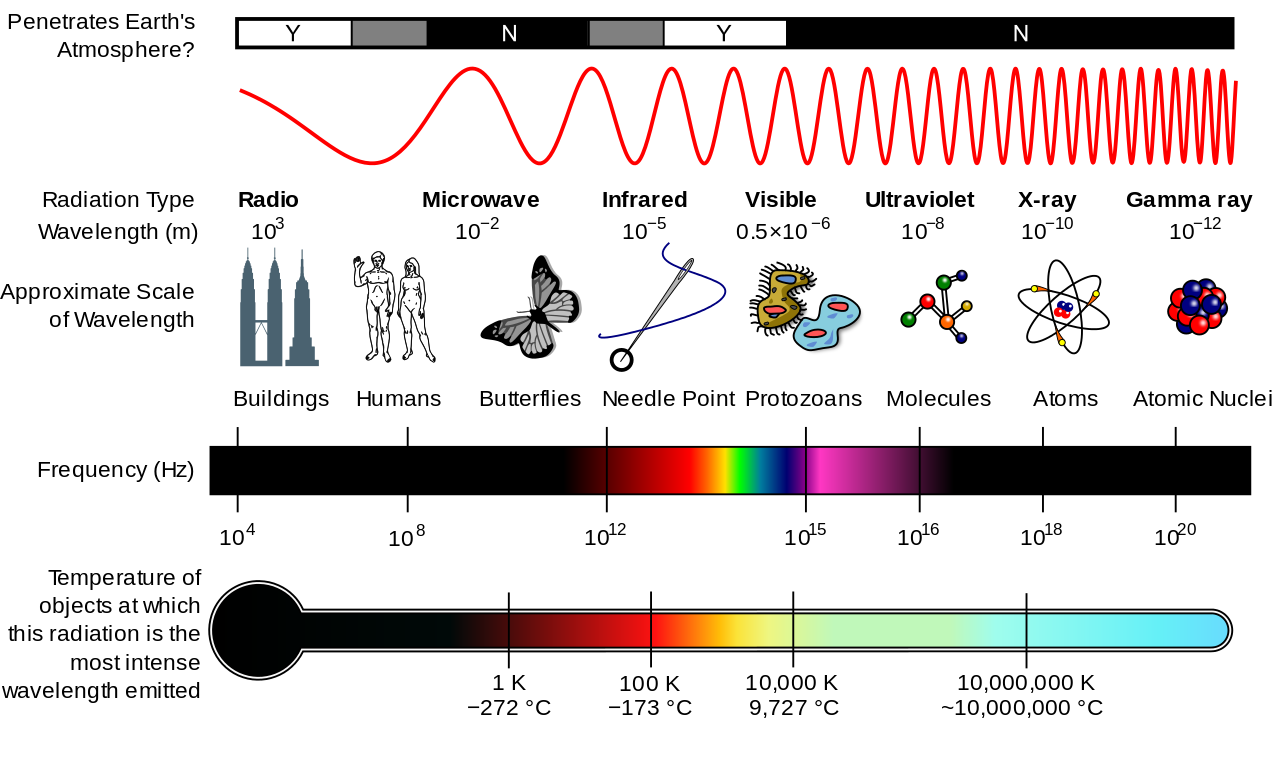
\includegraphics[width=.8\textwidth]{images/em_spectrum.png}
	\caption{An overview of properties and applications for a wide 
		range of photon energies.
		Radio-waves are at the lowest energies, gamma-rays 
		at the very highest energies.
		Visible light lies in between, technical 
		applications exist for all the shown wavelengths.
		Image from \cite{wiki_em}}
	\label{fig:em_spectrum}
\end{figure}


ENSTEHUNG ERKLÄREN -> synchroton, inverse compton
Erklärung aus func ray, kais diss zum Verständnis




Emitted $\gamma$-rays can be observed either directly
from outside the atmosphere via satellites or indirectly
via ground based gamma astronomy. In the later case
IACTs are used to detect electromagnetic showers induced
by the collision of high energy photons with particles in the atmosphere.
An example for direct observation could be the Fermi 
Gamma-Ray Space Telescope \cite{Atwood_2009},
an example for ground based observation could be the
MAGIC-experiment \cite{LORENZ2004339}.

\iffalse
\subsection{Neutrinos}
Even less affected by interactions on the way 
from the source to the earth are neutrinos ($\nu$).
Due to their small interaction cross sections and no electric charge, they 
suffer very little from absorption or deflection.
For very much the same reasons detecting neutrinos is much harder
than detecting photons or charged particles.

The small cross section requires to build huge detectors, 
the ICECUBE having a detector volume of \SI{1}{\kilo\meter^3}
\cite{Abbasi:2008aa}.
An illustration of the ICECUBE Neutrino Observatory
is shown in figure \ref{fig:icecube}.
\begin{figure}
	\centering
	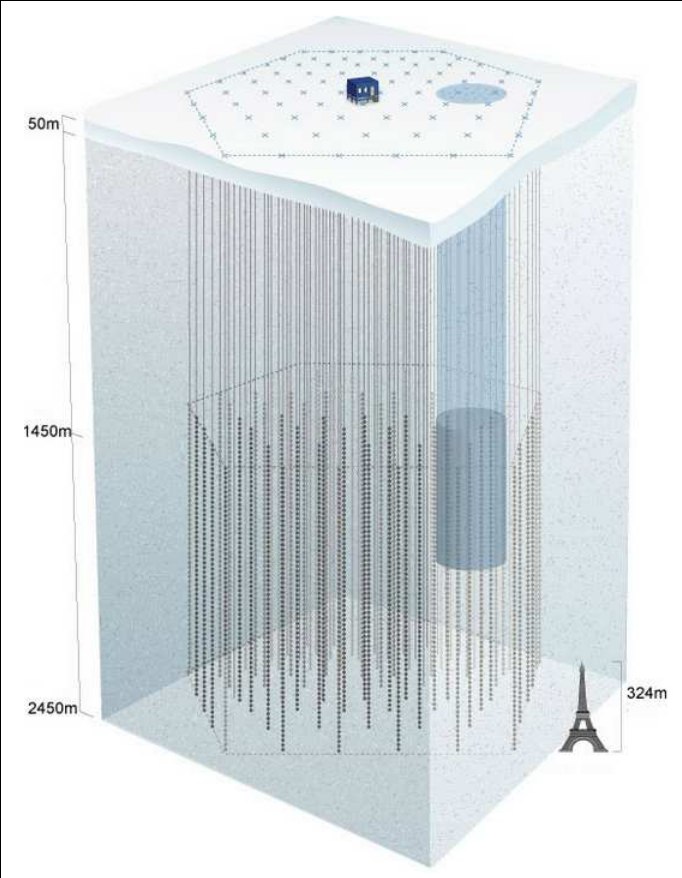
\includegraphics[width=0.8\textwidth]{images/icecube.png}
	\caption{icecube illustration, cite that \cite{Abbasi:2008aa}}
	\label{fig:icecube}
\end{figure}

\subsection{Gravitational waves}
Gravitational waves are the newest channel available for observation.
They are a direkt result from general relativity and occur
at certain constellations of very high masses, such as 
merging black holes.

An illustration of such an event is shown in figure \ref{fig:gravi_waves}. 
\begin{figure}
	\centering
	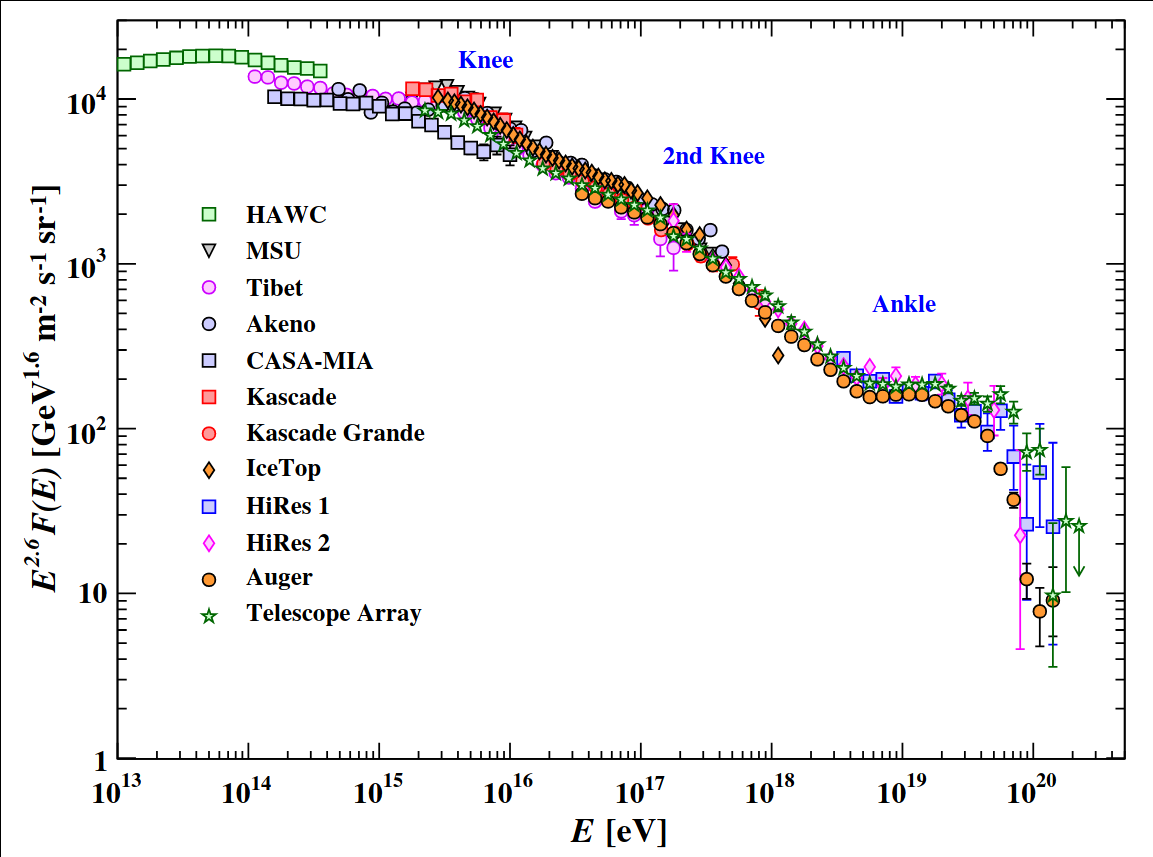
\includegraphics[width=0.8\textwidth]{images/cr_spectrum.png}
	\caption{images}
	\label{fig:gravi_waves}
\end{figure}


We can detect them using large size interferometers such as
the LiGO's three detectors (citation needed).
\fi

\section{Detection of gamma-rays with ground based telescopes}
The primary particles of gamma or cosmic rays cannot be 
observed with IACTs directly. Instead one can measure the secondary particles
that emerge from the particles interaction with matter.

If the primary particle energy is high enough, the resulting 
secondary
particles can interact with the atmosphere themself, thus starting a 
cascade of secondary particles.

Depending on whether the primary particle is 
a photon/electron/positron or a heavier particle such as a proton 
or iron core, the interactions vary.

This leads to a separation of electromagnetic and hadronic showers.
If the experiment is primarly looking for 
gamma rays, e.g. if measuring a known source like the Crab Nebula, 
the hadronic showers can be treated as background.
As hadronic showers get observed much more frequently, 
the identification of the primary particle type is a very important 
task, often times referred to as gamma-/hadron-separation.

To understand how these showers differ, we will have a very brief look
at the relevant interactions at the primary particle energies
we want to observe (above some  \SI{10}{\giga\electronvolt}.

\subsection{Electromagnetic showers}
Electromagnetic showers consist mainly of three types of particles:
\begin{enumerate}
	\item{Photons $\gamma$}
	\item{Electrons $e^-$}
	\item{Positrons $e^+$}
\end{enumerate}

The main interaction for high energy photons is pair 
production, generating an $e^+-/e^--$pair where the energy of 
the secondary particles equals the photon energy.
On the other hand high energy electrons (and positrons) lose 
most of their energy by radiation, leading to a photon with 
an energy close to the electron energy.

Only at lower particle energies other interaction forms show their impact,
with particle scattering and ionisation 
leading to more continous energy losses.

These assumptions lead to the most basic model of an 
electromagnetic shower, proposed by Bhabha and Heitler in 1937
\cite{doi:10.1098/rspa.1937.0082}.
MEHR HIER ERKLÄREN


Today monte carlo calculations get used to simulate the properties 
of particle showers in the atmosphere.
The most common software to model the athmospheric interactions is
CORSIKA \cite{Engel:2018akg}.

Although the energy losses are mainly negligible, 
the most important interaction for the detection with IACTs is 
cherenkov radiation: High energy charged particles pass through 
matter faster than the speed of light in the medium. This leads
to the emittance of near-visible photons that get detected 
in the telescopes camera. 


\subsection{Hadronic showers}
Hadronic shower include all the interactions known from 
electromagnetic showers, but add nuclear interactions on top.
These lead to non-negligible additional energy losses 
and the creation of secondary hadronic particles.

Approximations are more difficult to do and simulations 
become the only way to reasonably calculate shower behaviour.

At the end of the shower most particles have decayed into the 
lightest hadronic particles, pions ($\pi^0, \pi^+, \pi^-$), of which the neutral pions 
rapidly decay into photons.
\cite{bookap} (vlt gibts da bessere quellen) states that on average
roughly a third of the pions are neutral pions. This means that 
a third of the hadronic shower eventually becomes an electromagnetic
subshower.

Figures \ref{fig:gamma_shower} and \ref{fig:proton_shower}
show a comparison of simulated 
$\gamma$- and proton showers.

\begin{figure}
	\centering
	\begin{subfigure}{.7\textwidth}
  		\centering
  		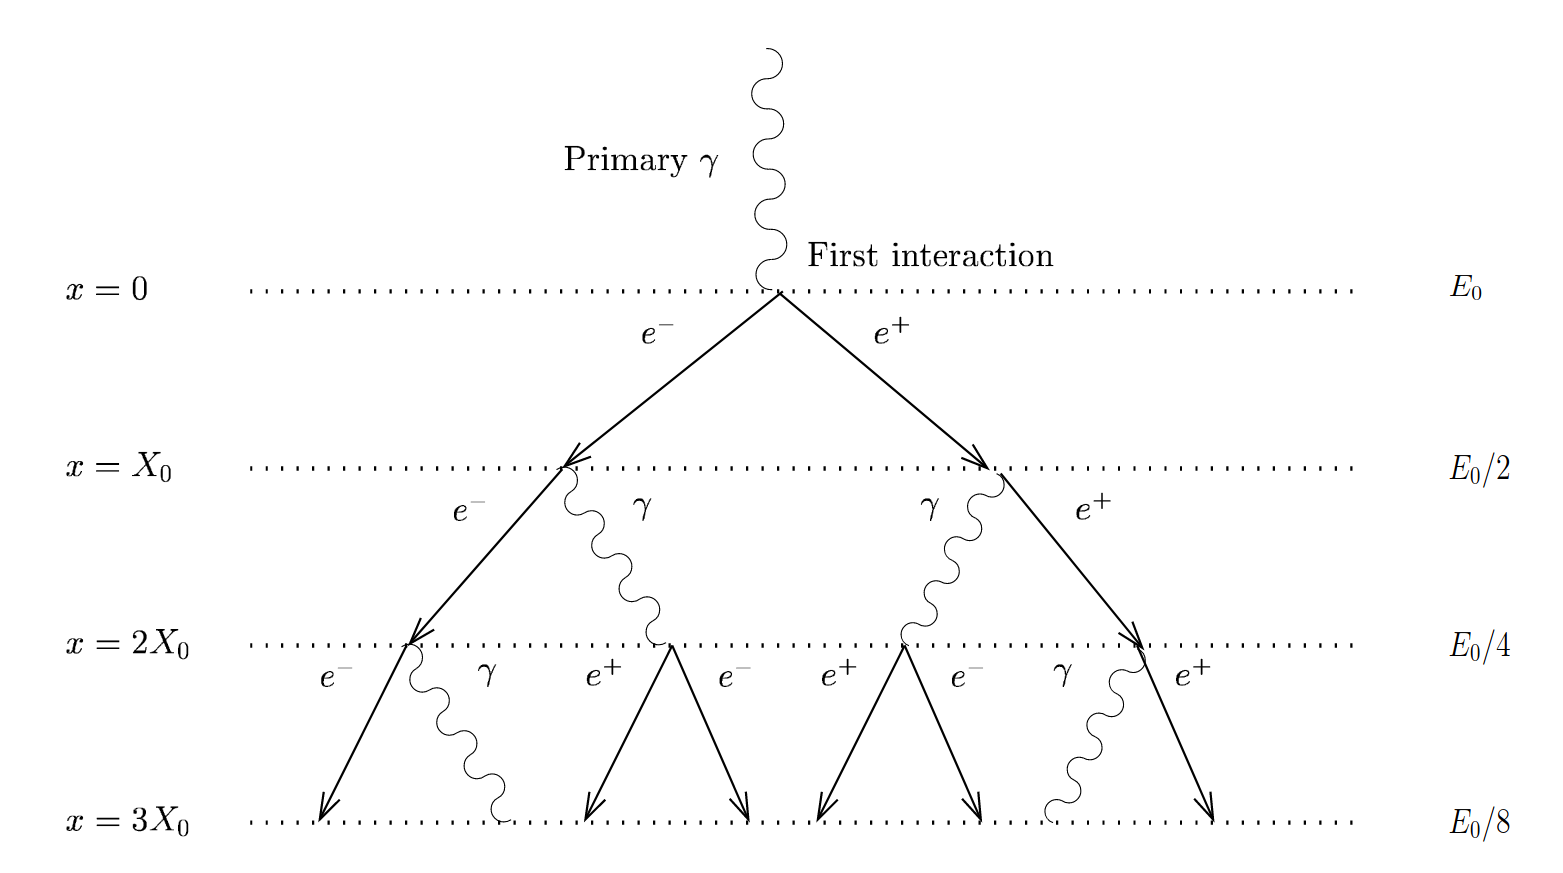
\includegraphics[width=\linewidth]{images/em_shower_illustration.png}
	\end{subfigure}%
	\begin{subfigure}{.3\textwidth}
 		\centering
		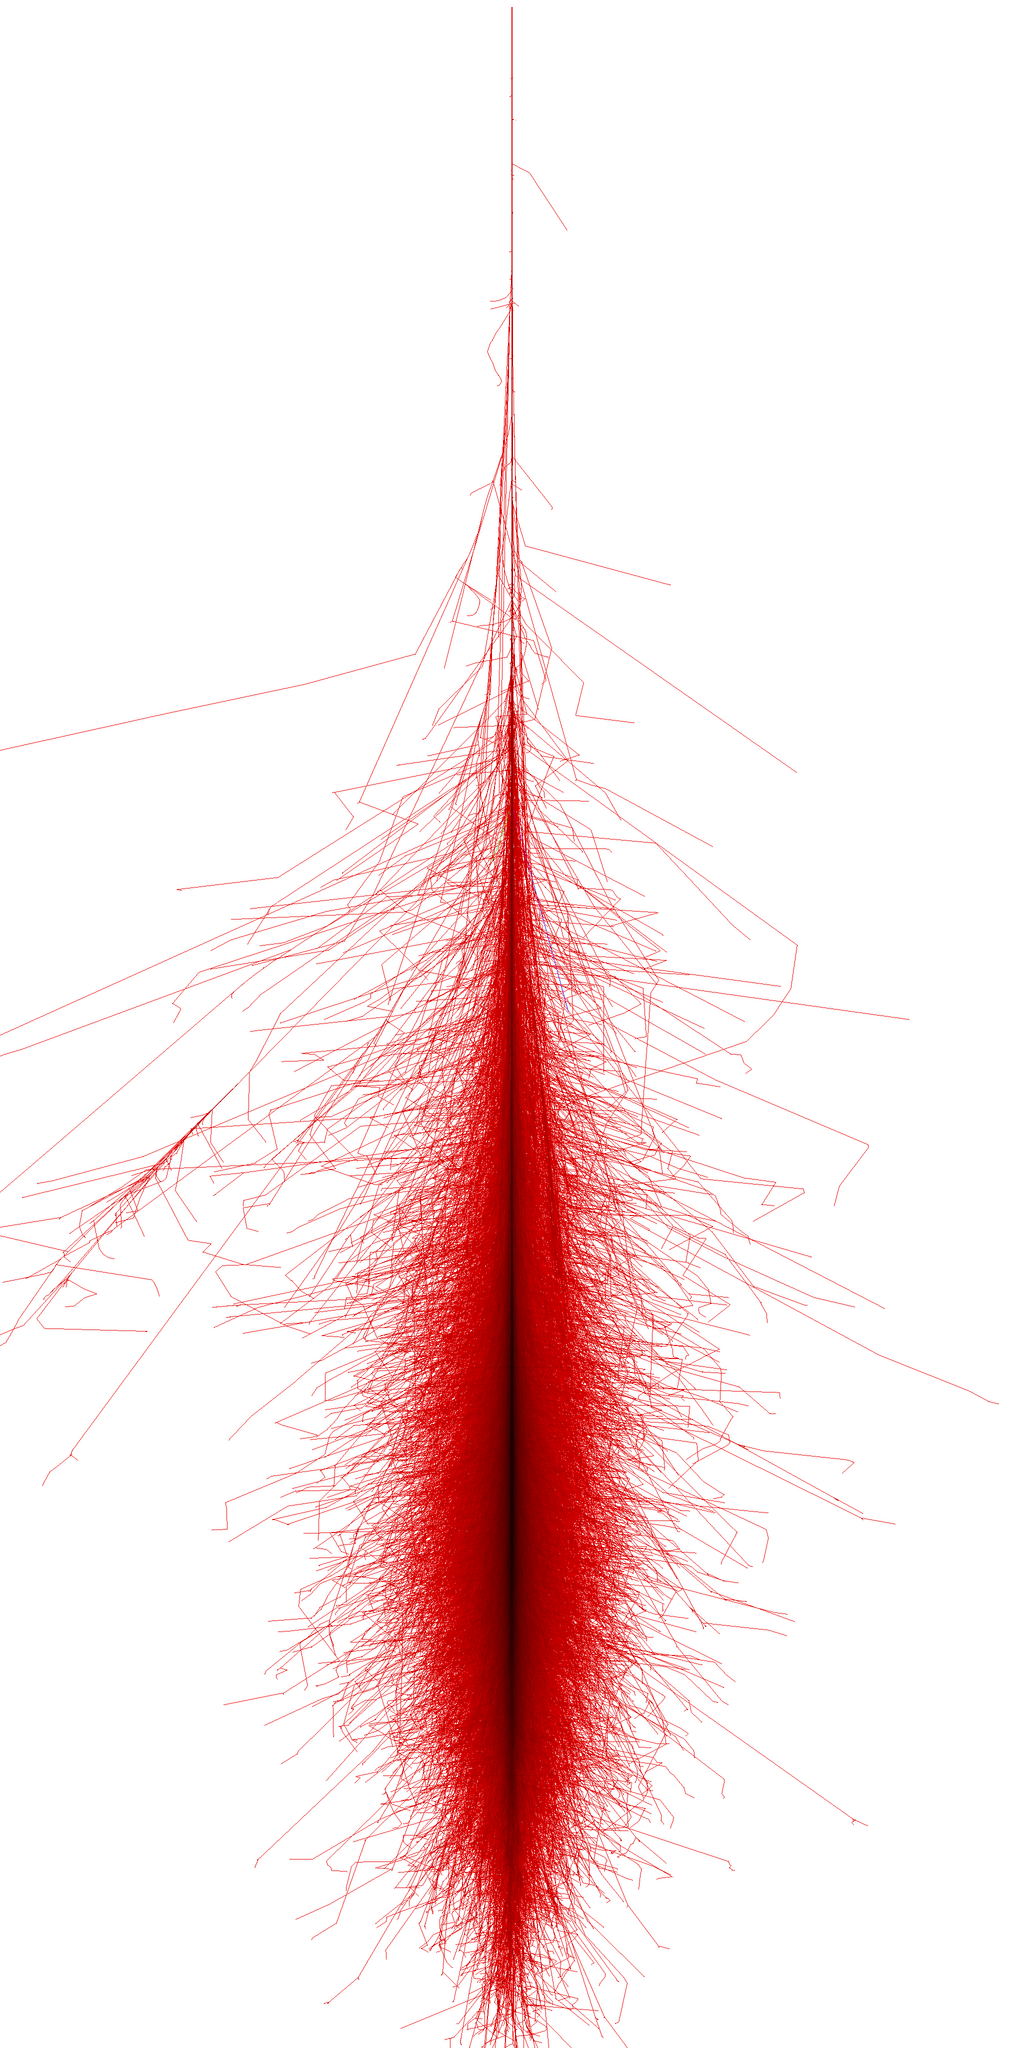
\includegraphics[width=.9\linewidth]{images/corsika_1tev_photon.png}
	\end{subfigure}
	\caption{Schematic illustration and simulated air showers as xz-projection.
		Left: A schematic illustration of the first epochs of the 
		Bethe-Heitler shower model with equal radiation lengths for
		bremsstrahlung and pair production.
		The image is taken from an inaugural thesis 
		by Stefan Funk \cite{funk_doctor}.
		Right: A \SI{1}{\tera\electronvolt} gamma-shower.
		The shower is very contained with only little extent perpendicular 
		to the shower direction (z-axis). The image is taken from 
		the CORSIKA-website \cite{corsika_showers}}
	\label{fig:gamma_shower}
\end{figure}

\begin{figure}
	\centering
	\begin{subfigure}{.7\textwidth}
  		\centering
  		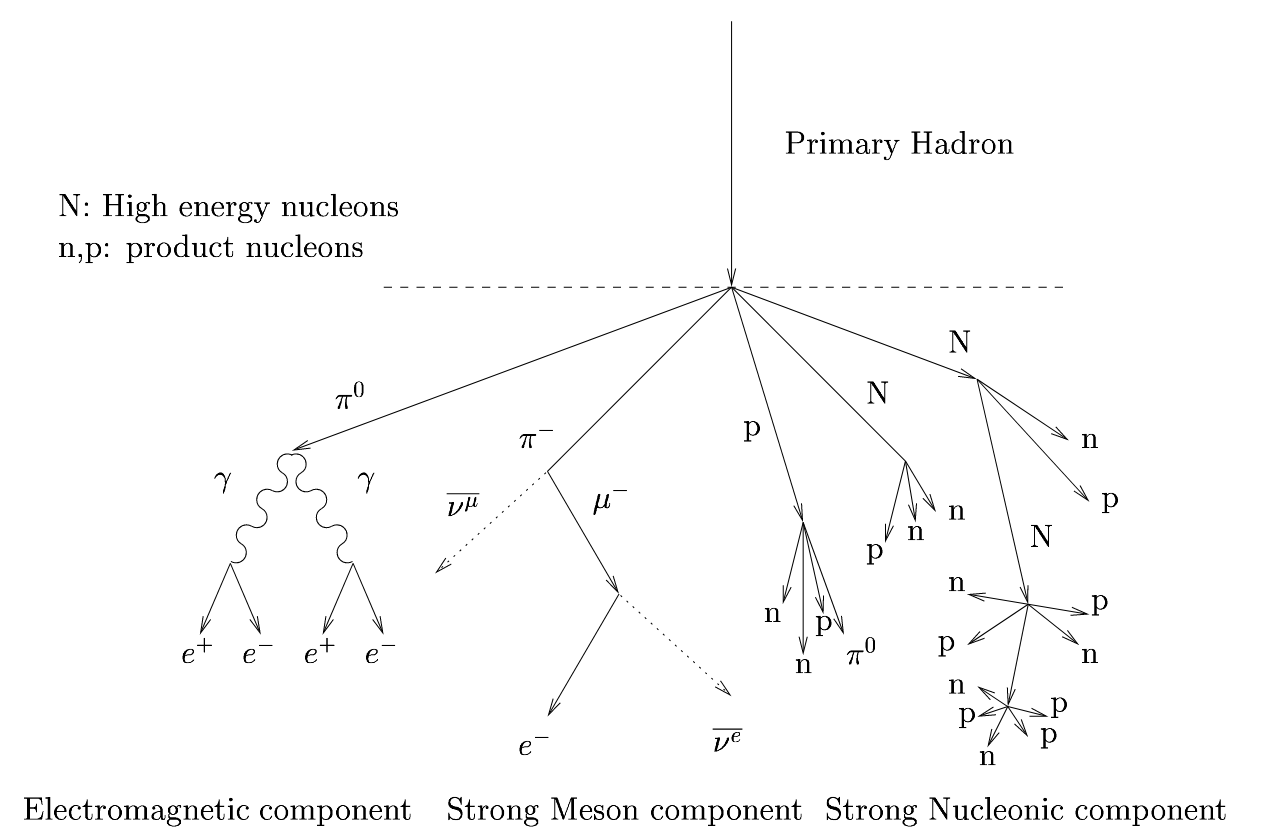
\includegraphics[width=\linewidth]{images/hadron_shower_illustration.png}
	\end{subfigure}%
	\begin{subfigure}{.3\textwidth}
 		\centering
		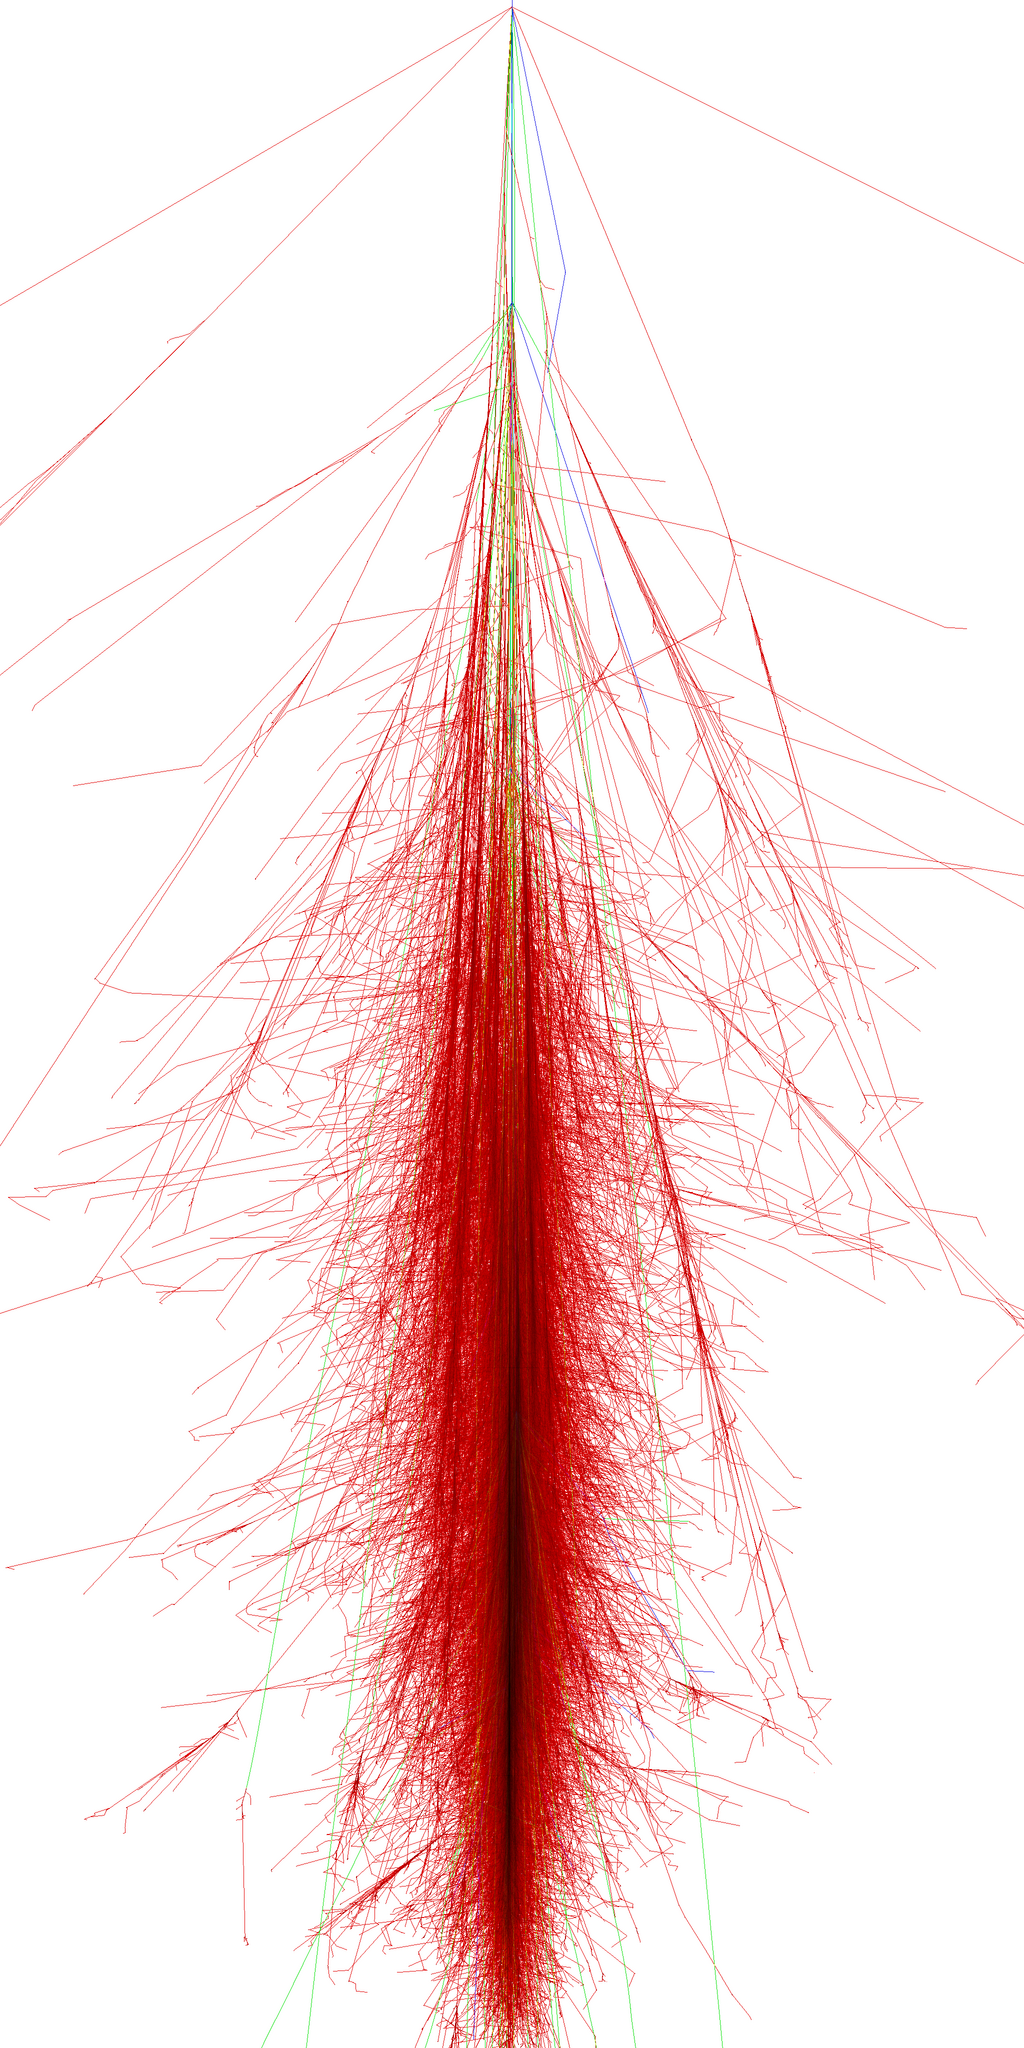
\includegraphics[width=.9\linewidth]{images/corsika_1tev_proton.png}
	\end{subfigure}
	\caption{Schematic illustration and simulated air showers as xz-projection.
		Left: A purely qualitative,
		schematic illustration of the generation of a hadronic shower.
		It shows how the primary hadron generates different subshowers
		with vastly different particles.
		The image is taken from an inaugural thesis 
		by Stefan Funk \cite{funk_doctor}.
		Right: A \SI{1}{\tera\electronvolt} proton-shower.
		The shower is less contained than the gamma shower of equal energy in 
		figure \ref{fig:gamma_shower}.
		The image is taken from 
		the CORSIKA-website \cite{corsika_showers}}
	\label{fig:gamma_shower}
\end{figure}

\subsection{Measuring events}
As stated earlier, IACTs measure particle showers by their emittance of cherenkov 
light. The cherenkov light covers a huge area on the floor (rephrase).

Single photons get collected by the mirror of a telescope (or a composition of 
multiple smaller mirrors) and projected onto a camera system mounted some 
meters above the mirror.
With this setup IACTs usually reach a field of view of 
a few degree (magic: wert, zitat, hess: wert, zitat, veritas: wert, zitat)
Figure \ref{fig:iact_mirror_camera} illustrates this 
setup.


\begin{figure}
	\centering
	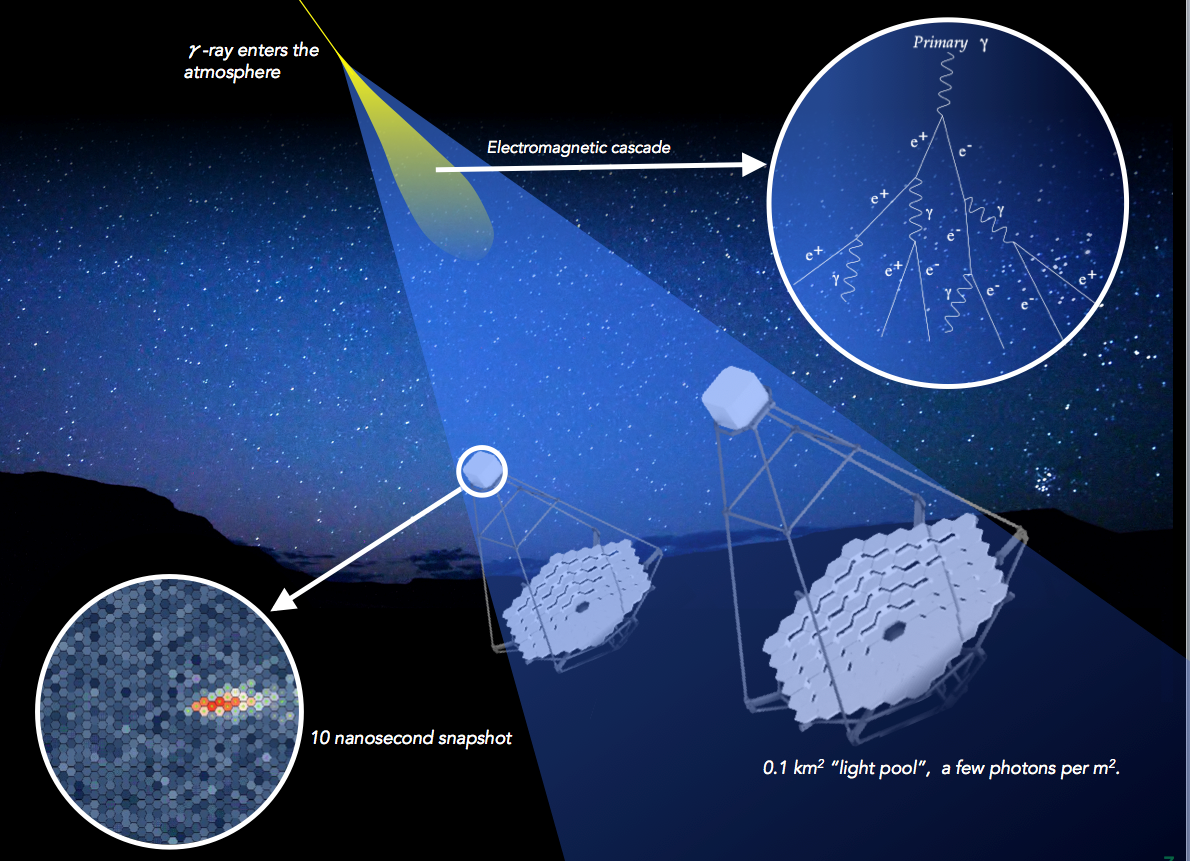
\includegraphics[width=0.6\textwidth]{images/cta47.png}
	\caption{A schematic illustration of the working principles of 
	a setup of two IACTs:
	A $\gamma$-ray produces an air shower in the atmosphere
	that points roughly towards the telescopes.
	Cherenkov light from the air shower 
	hits the mirrors and gets focussed into a camera mounted on top.
	An illusration of the resulting image after after integrating 
	\SI{10}{\nano\second} of the waveform at the time the shower hits
	can be seen in the left bottom corner.
	Any further reconstruction steps are left out.
	Image from \cite{cta_web}}.
	\label{fig:iact_mirror_camera}
\end{figure}


Upon detection of a shower and performing the low-level analysis,
the usual tasks of a high-level analysis include reconstructing 
three key properties of the primary particle:
\begin{enumerate}
	\item{Particle type (mostly photon or hadronic)}
	\item{Primary particle energy}
	\item{Direction (leading to the source position)}
\end{enumerate}

This usually involves describing the 
shower image as an ellipse and calculating the hillas parameters.
The historical approach can be read up in 
a famous paper of A.M. Hillas \cite{hillas_params}.
This allows to describe the shower image with only a handful of parameters.

In most cases the reconstruction can be improved heavily by cleaning the image first.
Figure \ref{fig:shower_cleaning} shows a simulated $\gamma$-induced shower image
in the camera of the Large Sized Telescope (LST, see section \ref{sec:lst} for more details of the telescope)
before and after cleaning.

\begin{figure}
	\centering
	\begin{subfigure}{.4\textwidth}
  		\centering
  		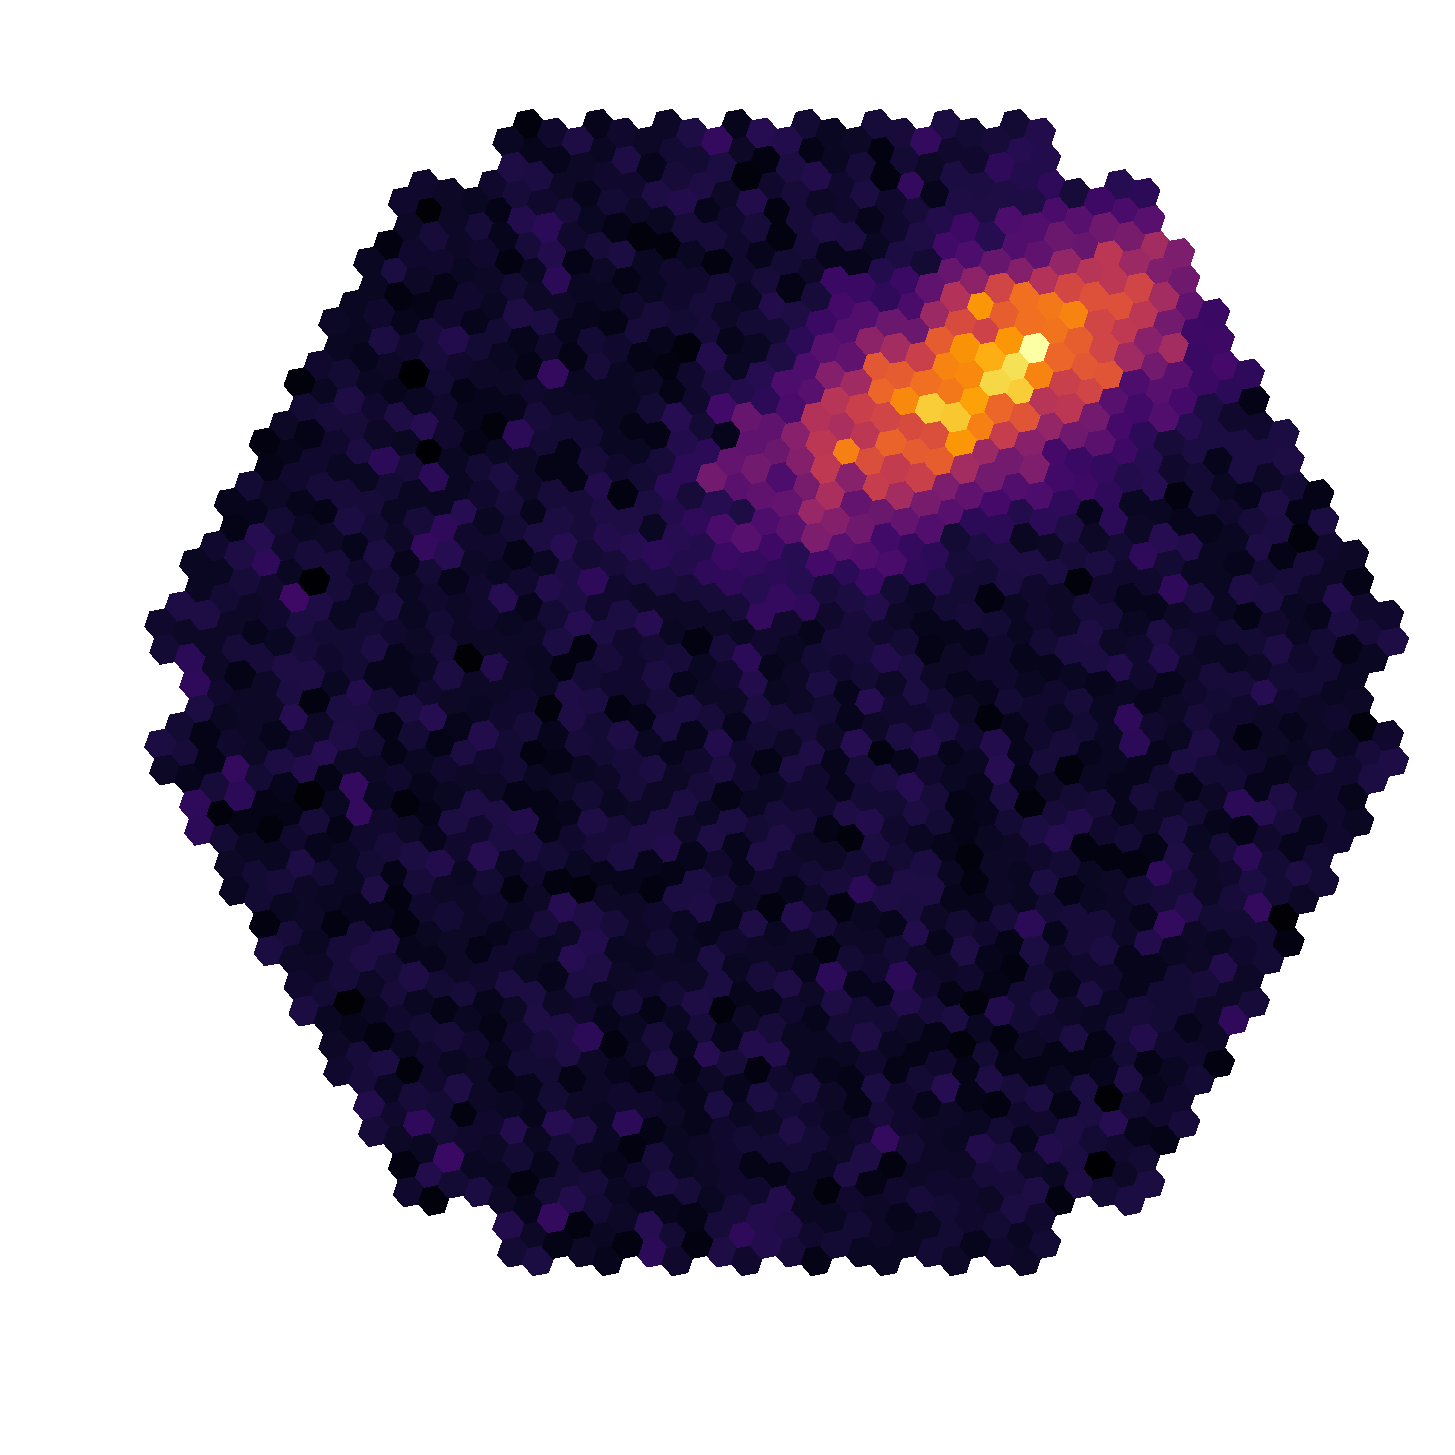
\includegraphics[width=\linewidth]{Plots/hillas_raw.pdf}
	\end{subfigure}%
	\begin{subfigure}{.4\textwidth}
 		\centering
		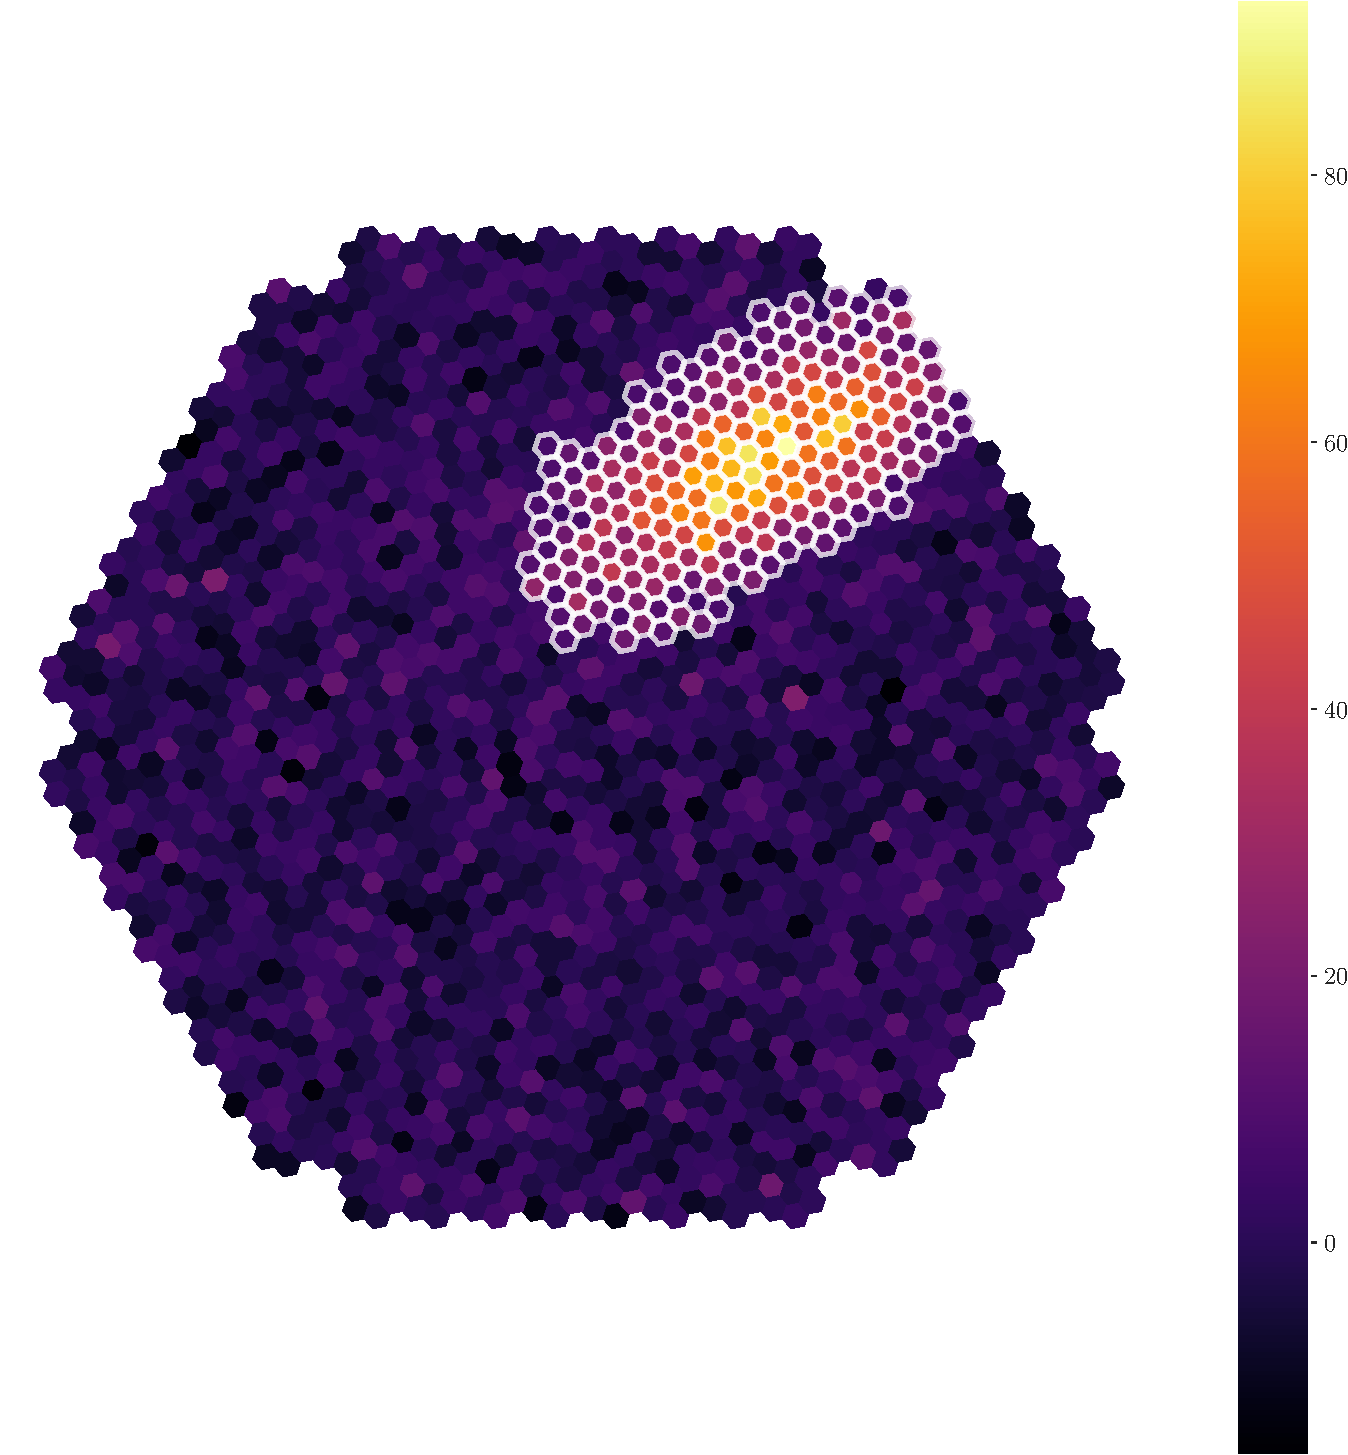
\includegraphics[width=\linewidth]{Plots/hillas_cleaned.pdf}
	\end{subfigure}
	\caption{A simulated gamma-shower in the camera of a LST.
		The pixel colors show the intensity as integrated 
		waveform in each pixel. The left image 
		shows the signal directly after
		the waveform integration, in the right image
		a cleaning-algorithm has been 
		applied. The noise in the non-signal pixels is gone,
		improving the analysis.
		This image is heavily idealized, real shower images 
		can be much harder to clean properly.}
	\label{fig:shower_cleaning}
\end{figure}

From the reconstructed image, the hillas parameters can be calculated.
An illustration with the hillas-ellipse on top of the camera image 
for the same image can be seen in figure \ref{fig:hillas_params}.

\begin{figure}
	\centering
	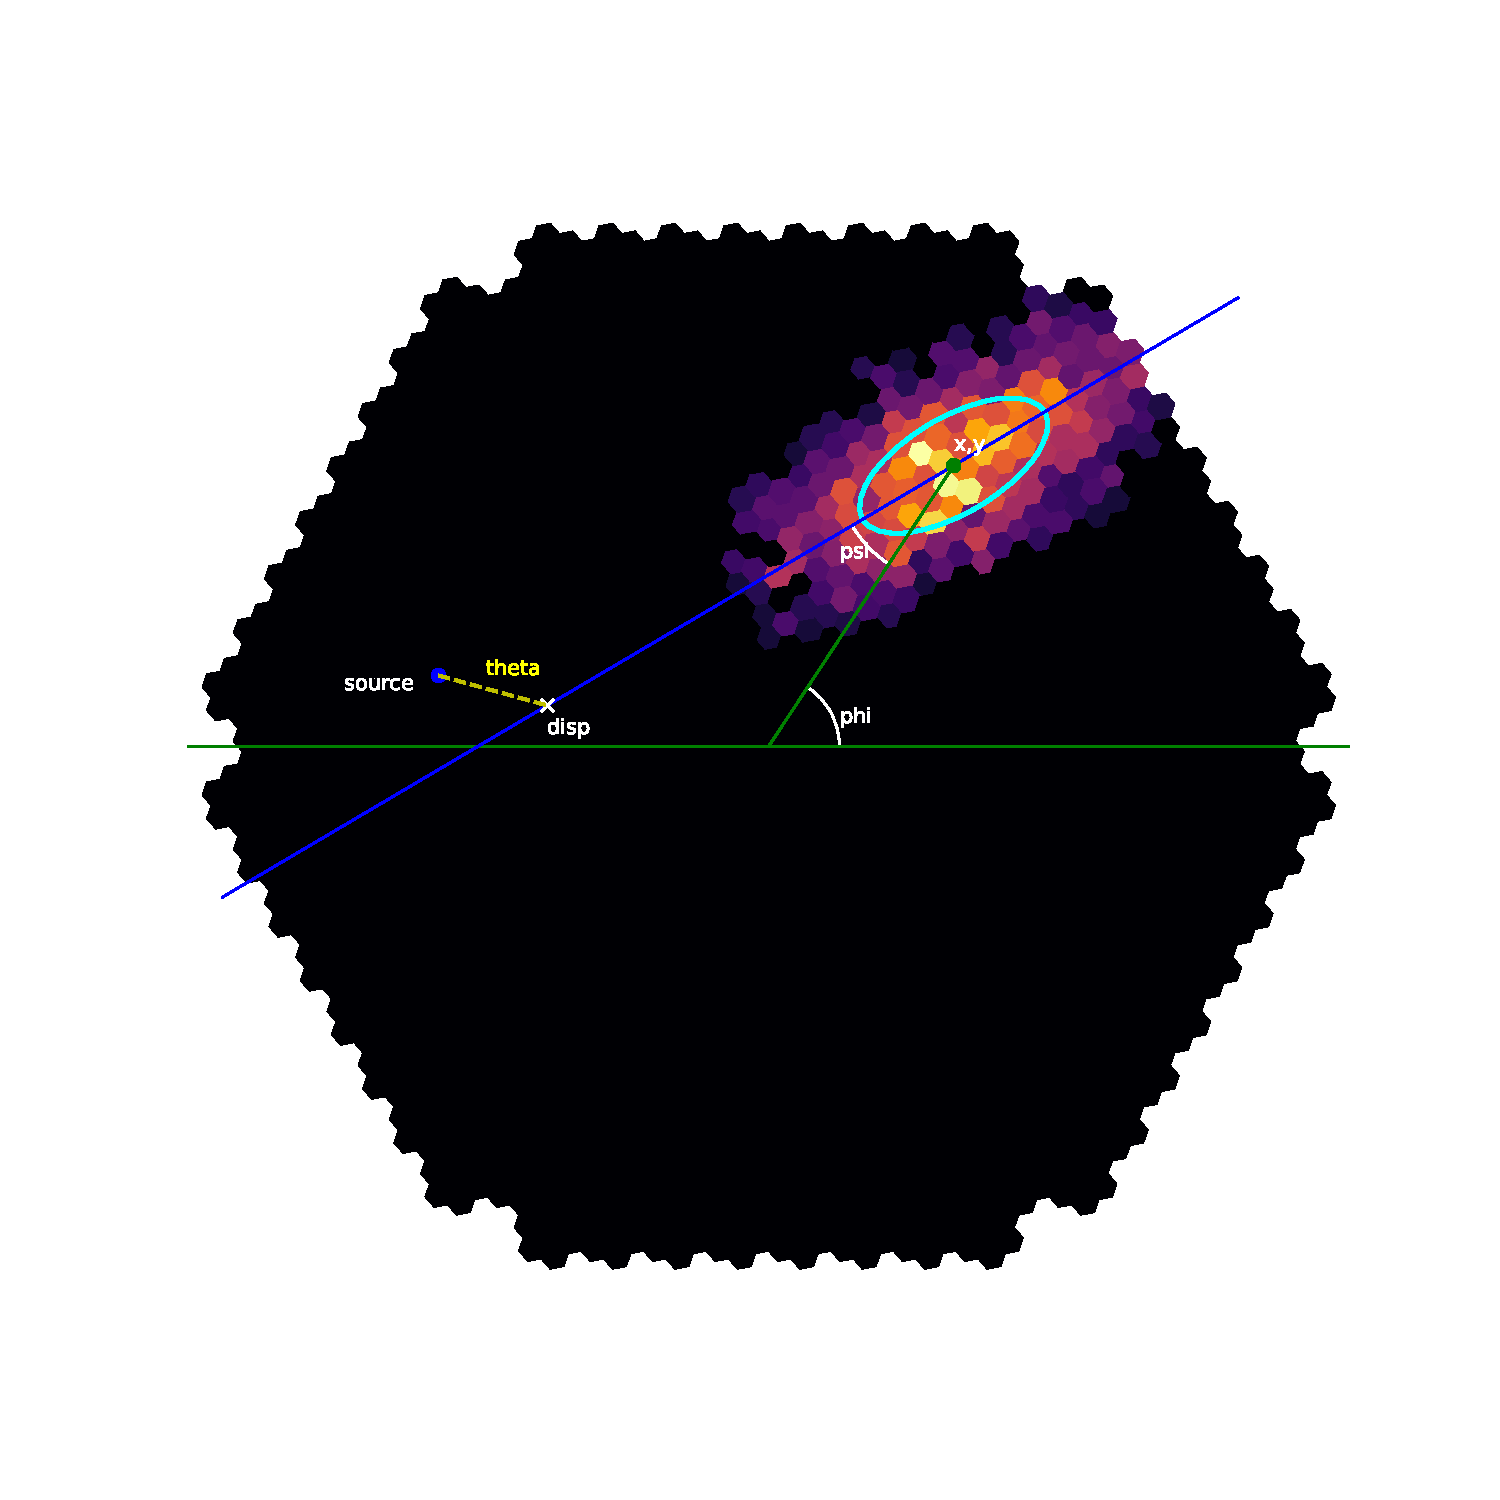
\includegraphics[width=.5\textwidth]{Plots/hillas_complete.pdf}
	\caption{The same cleaned shower-image as in figure \ref{fig:shower_cleaning}
	with the hillas-parameters calculated and marked in the camera frame.
	Two angles $\phi$ and $\psi$ describe the direction of the 
	main shower axis, two coordinates $x$ and $y$ describe the position of 
	the center of gravity of the image in the camera frame.
	The shower axis constrains the reconstruction of the source position to a 
	point on a line. Via the DISP-method two possible points remain.
	This is sometimes refferd to as the head-tail-ambiguity.
	}
	\label{fig:hillas_params}
\end{figure}

With the hillas parameters calculated, the reconstruction of the 
primary particles properties can be done.

In first order one can predict the shower origin by 
transforming the center of gravity (cog) of the image onto the sky plane.
More sophisticated methods assume that the 
center of gravity is displaced relative to the
real source position depending on the angle the photon arrived at the telescope.
With higher angles the shower ellipse gets more eccentric as well.
The ellipsicity of the ellipse is thus a measure for the displacement of the true 
source position.

If one assumes the true source position to be on the main shower axis of the ellipse,
finding this position simplifies to finding a single point on the main shower axis.
This is often times referred to as DISP-method,
which in a basic form was already getting used at 
the WHIPPLE-telescope in ???? \cite{???}.

Monoscopic experiments also need to resolve the head-tail-ambiguity:
Knowing the distance from the cog leaves two possible points, one on either side 
of the ellipse.

Stereoscopic experiments can resolve this ambiguity by combining the images from 
multiple telescopes, as can be seen in figure \ref{fig:stereo_shower}.

\begin{figure}
	\centering
	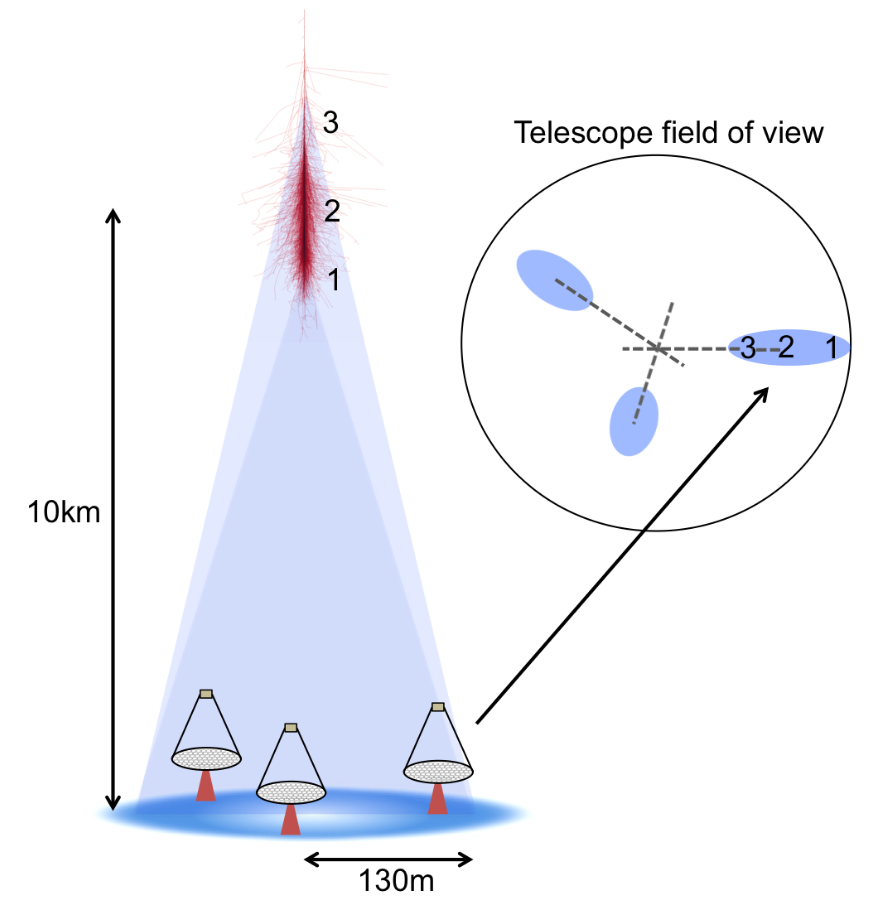
\includegraphics[width=0.5\textwidth]{images/stereo_shower.png}
	\caption{An illustration of an air shower captured with multiple telescopes.
		Upper right: Each telescope captures an elliptic image.
		The image axes get intersected to reconstruct the arrival direction
		of the primary particle. This resolves the head-tail-ambiguity
		by using the information of all telescopes at the same time
		and removes the need of calculating the displacement altogether by
		assuming the intersection point as true source position.
		However, using the displacement still improves the reconstruction 
		in some cases \cite{some magic paper states that }.
	    Image taken from \cite{holder2015atmospheric}.}
	\label{fig:stereo_shower}
\end{figure}

The primary particle energy is mostly described by the contained light in the image combined with 
an estimate of how much of the light missed the camera. 

The particle type can be reconstructed 
by looking at the image shape.
As we saw earlier, $\gamma$ and hadronic showers have different properties, 
resulting in different images. The assumption of a single, elliptic signal
area only works reasonably well for $\gamma$-showers.
A representation of different shower types can be seen in \ref{fig:compare_showers}

\begin{figure}
	\centering
	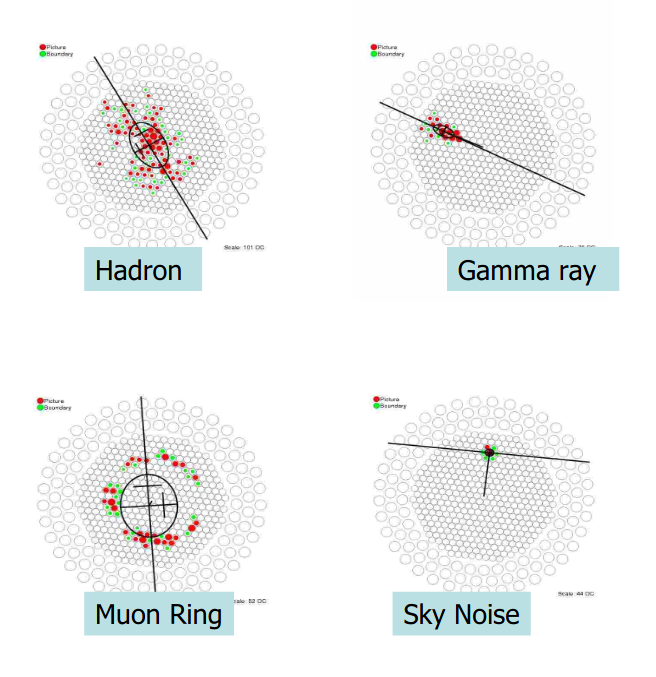
\includegraphics[width=.5\textwidth]{images/shower_types.png}
	\caption{A comparison of different shower types as seen 
	by the Whipple telescope during later stages of its observation
	when it had a multiple pixel camera installed.
	More about the the history of the Whipple telescope in section
	\ref{sec:1stgen_iact}. The general look of the shower types 
	is the same for all IACTs.
	Hadronic showers are more separated than gamma showers and tend to
	form multiple clusters in the camera.
	Muons often times produce ring-like images in the camera (WHY?).
	Background noise can take any form, but is usually constarined to very small
	areas as the pixel values are mostly random and uncorellated. 	
	Image taken from an introduction lecture by Albrecht Karle \cite{icecube_showers}.}
	\label{fig:compare_showers}
\end{figure}
